\chapter{Simulation-Based Inference for Polarization Estimation}
\label{chap:sbi}

\section{Introduction}
\S\ref{sec:polest} explained how to best estimate polarization parameters $(p_0, \theta_0)$ given a group of reconstructed photoelecton emission angles $\{\hat{\theta}_i\}^N_{i=1}$. This section explains how to best estimate polarization parameters given a group of reconstructed photoelecton emission angles \textit{and their associated uncertainties} $\{\hat{\theta}_i, \hat{\kappa}_i\}^N_{i=1}$. These uncertainties can vary for different individual emission angles; the measurements are heteroskedastic.
Emission angles with larger uncertainties should contribute less to the final polarization parameter estimates. In theory, this section need not use DNNs and the methods described can be used for any track reconstruction method that provides (trustworthy) emission angle uncertainties; the uncertainties can be parameterized by any appropriate distribution. In practice, the predicted emission angle uncertainties come from deep ensembles and the uncertainties are assumed to follow a von Mises family of distributions. 

\section{Modulation factor}
To develop a polarization estimation method that incorporates emission angle uncertainties, it is essential to specify how these uncertainties affect the recovered emission angle distribution eq.~\ref{eqn:likelihood}. For a source with polarization parameters $(p_0, \theta_0)$, the true photoelectron emission angles follow the distribution eq.~\ref{eqn:likelihood}, while the recovered or measured emission angles follow eq.~\ref{eqn:likelihoodmu}. The difference between the two is captured by the modulation factor $\mu$. The modulation factor summarizes the effect of uncertainty in individual emission angle measurements.  
%The link is the modulation factor $\mu$.

Consider a single emission angle measurement $\hat{\theta}_i$. Since track reconstruction methods are imperfect and contain sources of error (even DNN based ones as was shown in \S\ref{chap:nn}), $\hat{\theta}_i$ can be considered a random variable:
\begin{equation}
    \hat{\theta}_i = \theta_i + \epsilon_i
\end{equation}
where $\theta$ is the true emission angle, which follows the distribution eq.~\ref{eqn:likelihood}, and the measurement error $\epsilon_i$ is a random variable with  
\begin{equation}
\label{eqn:properties}
    \mathbb{E}[\epsilon_i] = 0, {\rm Var}[\epsilon_i] = \sigma^2_i, p(\epsilon_i=0) = p(\epsilon_i = 2\pi) 
\end{equation}
This assumes the $\hat{\theta}_i$ estimate is unbiased; reasonable given both the deep ensemble and moment analysis in \S\ref{sec:perform} are for the most part unbiased estimators. 
The specific distribution for $\epsilon_i$ will depend on the track reconstruction method, but all distributions should follow the properties in eq.~\ref{eqn:properties}: be unbiased, have a finite variance, and be periodic, since $\hat{\theta}$ itself is periodic. 

For any $\epsilon_i$ distribution with the above properties, it is possible to find the distribution for $\hat{\theta}_i$ as the convolution of the $\theta_i, \epsilon_i$ distributions:
\begin{equation}
    p(\hat{\theta}_i\mid p_0,\theta_0,\sigma_i^2) = \frac{1}{2\pi} \big(1 + \mu_ip_0\cos[2(\hat{\theta}_i - \theta_0)] \big),
    \label{eqn:individual}
\end{equation}
where $0 \leq \mu_i \leq 1$, $\mu_i(\sigma^2_i)$ and $\mu_i(\sigma_i^2 = 0) = 1$.
In other words, the distribution of estimators $\hat{\theta}_i$ are the same as the distribution of the true values $\theta_i$ but with a reduced individual modulation factor $\mu_i(\sigma^2_i)$ that depends on the measurement error $\sigma^2_i$. The measurement noise will blur the sinusoidal modulation signal by a factor $\mu_i$ for the specific event $i$. 

The final distribution for a set of recovered emission angles $\{\hat{\theta}_i\}^N_{i=1}$ can now be simply formulated as an equal mixture model of the distributions of all individual recovered emission angles, eq.\ref{eqn:individual}:
\begin{eqnarray}
    p(\hat{\theta}\mid p_0,\theta_0) =& \frac{1}{N}\sum_{i=1}^N\frac{1}{2\pi} \big(1 + \mu_ip_0\cos[2(\hat{\theta} - \theta_0)] \big),\\
    =& \frac{1}{2\pi} \big(1 + \big( \frac{1}{N}\sum_{i=1}^N \mu_i \big)p_0\cos[2(\hat{\theta} - \theta_0)] \big),\\
    =& \frac{1}{2\pi} \big(1 + \mu p_0\cos[2(\hat{\theta} - \theta_0)] \big).
    \label{eqn:mix}
\end{eqnarray}
Thus, the final modulation factor of a set of emission angles with varying individual measurement errors $\{\hat{\theta}_i, \sigma_i^2\}^N_{i=1}$ is an average over all individual modulation factors 
\begin{equation}
    \mu = \frac{1}{N}\sum_{i=1}^N \mu_i(\sigma_i^2),
\end{equation}
where individual modulation factors each depend on the individual measurement errors $\sigma_i^2$.

For a specific example of an individual modulation factor, consider the case where $\epsilon_i$ is VM(0,$\kappa_i$) between $[0,\pi]$. This is the uncertainty distribution learned by the deep ensembles in \S\ref{chap:nn}. 
\begin{equation}
p(\epsilon_i) = \frac{1}{2\pi I_0(\kappa_i)}\exp(\kappa_i\cos2\epsilon_i).
\label{eqn:vm}
\end{equation}
This distribution meets all the assumptions stipulated in eq.~\ref{eqn:properties}. Evaluating the convolution of the $\theta$ (eq.\ref{eqn:likelihood}) and $\epsilon$ (eq.\ref{eqn:vm}) distributions, one finds
\begin{equation}
    p(\hat{\theta}_i\mid p_0, \theta_0, \kappa_i) = \frac{1}{2\pi} \big(1 + \frac{I_1(\kappa_i)}{I_0(\kappa_i)}p_0\cos[2(\hat{\theta}_i - \theta_0)] \big).
    \label{eqn:vm_hat}
\end{equation}
Comparing to eq.~\ref{eqn:individual}
\begin{equation}
    \mu_i = \frac{I_1(\kappa_i)}{I_0(\kappa_i)},
    \label{eqn:weight_func}
\end{equation}
and the modulation factor for set of tracks $\{\hat{\theta}_i, \kappa_i\}^N_{i=1}$ is 
\begin{equation}
    \mu = \frac{1}{N}\sum_{i=1}^N \frac{I_1(\kappa_i)}{I_0(\kappa_i)},
\end{equation}


\section{Weighted maximum likelihood estimator}
In \S\ref{sec:polest}, it was assumed when estimating polarization parameters that the modulation factor is a constant, $\mu$. The previous section showed how the modulation factor arises from the measurement errors of many individual emission angle estimates. If individual uncertainties are known, rather than assuming these lead to one constant $\mu$, individual modulation factors can be directly incorporated into the likelihood function for the polarization parameters. 

With individual emission angle measurement errors known, the likelihood eq.~\ref{eqn:likelihood_stoks} can be expressed as a more informative likelihood:
\begin{equation}
    L(\{\hat{\theta}_i\}_{i=1}^N\mid\mathcal{Q},\mathcal{U}) =  \prod_{i=1}^N\frac{1}{2\pi} \big(1 + \mathcal{Q}\mu_i\cos2\hat{\theta}_i + \mathcal{U}\mu_i\sin2\hat{\theta}_i \big).
    \label{eqn:prob_stoks}
\end{equation}
Now each estimated emission angle $\hat{\theta}_i$ comes with its own individual modulation factor $\mu_i$, as opposed to a global $\mu$. This likelihood can be maximized in exactly the same way as eq.~\ref{eqn:likelihood_stoks}. Following \S\ref{sec:polest}, assuming $|\mathcal{Q}\mu_i| << 1$, $|\mathcal{U}\mu_i| << 1$, the maximum likelihood estimators for Stokes' parameters $(\mathcal{Q}, \mathcal{U})$ are now
\begin{equation}
    \hat{\mathcal{Q}} = \frac{2}{\sum_{i=1}^N\mu_i^2} \sum^N_{i=1}\mu_i\cos2\hat{\theta}_i,
    \label{eqn:qestw}
\end{equation}
\begin{equation}
    \hat{\mathcal{U}} = \frac{2}{\sum_{i=1}^N\mu_i^2} \sum^N_{i=1}\mu_i\sin2\hat{\theta}_i.
    \label{eqn:uestw}
\end{equation}
Following the notation in \citet{kislat_analyzing_2015} and \citet{peirson_towards_2021}, one can define the individual event weights
\begin{equation}
    w_i = \mu_i
\end{equation}
and the total modulation factor (now a weighted average)
\begin{equation}
    \mu = \frac{\sum^N_{i=1} w_i\mu_i}{\sum_{i=1}^N w_i} = \frac{\sum^N_{i=1} w_i^2}{\sum_{i=1}^N w_i}.
\end{equation}                                     
Then eqs.\ref{eqn:qestw},\ref{eqn:uestw} are 
\begin{equation}
    \hat{\mathcal{Q}} = \frac{2}{\mu\sum^N_{i=1}w_i} \sum^N_{i=1}w_i\cos2\hat{\theta}_i,
    \label{eqn:qestww}
\end{equation}
\begin{equation}
    \hat{\mathcal{U}} = \frac{2}{\mu\sum^N_{i=1}w_i} \sum^N_{i=1}w_i\sin2\hat{\theta}_i.
    \label{eqn:uestww}
\end{equation}
Now when estimating the polarization parameters, each event is weighted by its expected signal $w_i = \mu_i$. As in \S\ref{sec:polest}, \citet{kislat_analyzing_2015} derive the posterior distribution for estimators eqs.~\ref{eqn:qestww},\ref{eqn:uestww}. The posterior distribution in the weighted case is the same as eq.\ref{eqn:posterior} but now $N$ is replaced with
\begin{equation}
N_{\rm eff} = \frac{\big(\sum_{i=1}^N w_i\big)^2}{\sum_{i=1}^N w_i^2},
\end{equation}
the effective number of events. Because the posterior distribution has changed, now
\begin{equation}
    \label{eqn:mdpw}
    {\rm MDP}_{99} = \frac{4.29}{\mu \sqrt{N_{\rm eff}}}.
\end{equation}
Weighting events reduces the total number of events contributing to a measurement of the polarization parameters, making $\sqrt{N_{\rm eff}}$ smaller, but it increases the modulation factor $\mu$ by more. Overall the MDP$_{99}$ is reduced, improving the polarization measurement. Since $w_i = \mu_i$ is the maximum likelihood estimator, this is the optimal event weighting scheme. It is also possible to arrive at this conclusion in reverse: starting with weighted estimators eq.~\ref{eqn:qestww},\ref{eqn:uestww} and MDP$_{99}$, eq.\ref{eqn:mdpw}, \citet{peirson_towards_2021} prove that $w_i = \mu_i$ minimizes the MDP$_{99}$, or equivalently maximizes the signal-to-noise ratio. 

\begin{figure}[t]
\centering
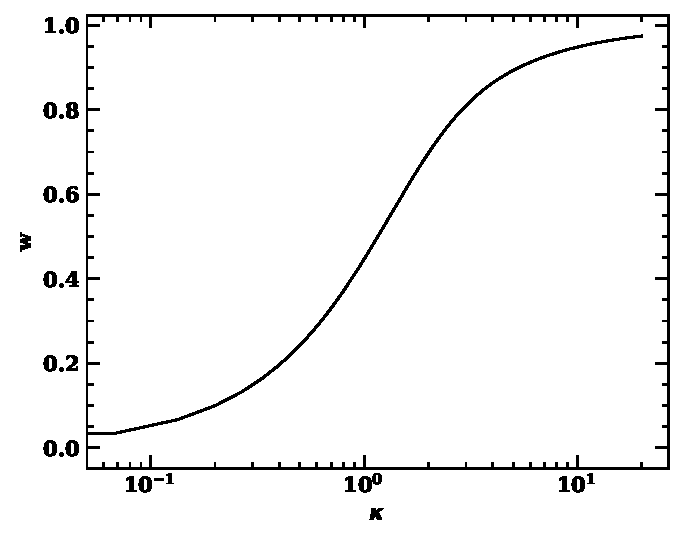
\includegraphics[scale=.8]{figures/weight.pdf}
\caption{Modulation factor or optimal event weight as a function of von Mises concentration parameter $\kappa$. Th function is monotonic, higher concentration parameters are always weighted more. }
\label{fig:weight}       % Give a unique label
\end{figure}

\subsection{Deep ensembles}
A DNN approach to track reconstruction using deep ensembles gives accurate estimates of individual VM uncertainties $\kappa_i$, \S\ref{sec:perform}. If measurement uncertainties are VM, individual modulation factors are given by eq.~\ref{eqn:weight_func}. 
Then, for a set of deep ensemble predicted emission angles and uncertainties, $\{\hat{\theta}_i, \hat{\kappa}_i\}^N_{i=1}$, weighted maximum likelihood estimators for the polarization parameters eq.~\ref{eqn:qestww},\ref{eqn:uestww} should use
\begin{equation}
\label{eqn:modw}
    w_i = \mu_i = \frac{I_1(\hat{\kappa}_i)}{I_0(\hat{\kappa}_i)}.
\end{equation}
Fig.~\ref{fig:weight} plots the optimal weighting (or equivalently, the modulation factor) as a function of $\kappa$. As expected, $0 \leq \mu_i \leq 1$ and an increasing concentration parameter $\kappa$ (decreasing uncertainty) always increases the event weight.

% Summary of the full pipeline...
% By using deep ensembles to predict ....
\section{Performance}
\label{sec:perform2}
It is now possible to compare the full polarimetery data analysis pipeline for a DNN approach with the classical moment analysis. Track reconstruction, step 1 of the pipeline, has already been compared in \S\ref{sec:perform}; this section will reveal how both track reconstruction improvements and uncertainty estimation affect polarization recovery. The quality of polarization recovery is measured by the MDP$_{99}$, eq.\ref{eqn:mdpw}. 

\begin{figure}[t]
\centering
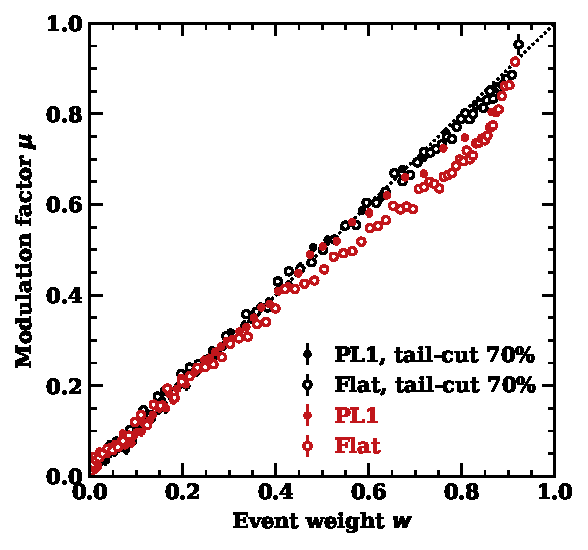
\includegraphics[scale=.8]{figures/mu100_v_W2_text.pdf}
\caption{Measured $\mu$ as a function of deep ensemble event weight $w$ for large test data sets of $1-10$keV simulated events. Each $\mu$ bin contains 20,000 individual track events. Closed circles represent a PL1 source ($dN/dE = E^{-1}$) convolved with IXPE's effective area, open circles a flat spectrum. Spectra with tail event cuts applied are in black, and full spectra in red.}
\label{fig:weight2}       % Give a unique label
\end{figure}

\subsection{Weights}
Before comparing methods, it is important to confirm that individual modulation factors $\mu_i$ (or weights $w_i$) predicted by the deep ensemble for each event, eq.\ref{eqn:modw}, are accurate. This can be checked by observing a $100\%$ polarized source and grouping events with same predicted $\mu_i$, then empirically measuring the modulation factor $\mu$ of the group with eq.\ref{eqn:p}. The measured and predicted $\mu$ should always match.

Fig.~\ref{fig:weight2} gives the measured modulation factor $\mu$ as a function of deep ensemble predicted weights $w_i = \mu_i$ for two polarized IXPE datasets with $1.5 \times 10^6$ events.
Any deviation from $y=x$ means the deep ensemble predicted uncertainties are imperfect. When most tail events are removed using a DNN tail cut, \S\ref{sec:removetail}, the deep ensemble predicted weights are close to perfect and show minimal spectral dependence. If tail events are allowed to remain in the spectrum, deep ensemble weights stray from the optimal MLE for highly weighted events. This is because it is difficult for the deep ensemble to learn the appropriate uncertainties $\hat{\kappa}$ for tail events, \S\ref{sec:perform}.
The effect is reduced for the PL1 spectrum where there are fewer high energy events and thus fewer tail events.



\begin{table}[t]
\centering
\begin{tabular}{@{}l l l @{}}
\toprule
{\textbf{Spectrum}}&{\textbf{Method}}&MDP$_{99}$(\%) \\
% & \multicolumn{3}{c|}{$\lambda=1$}\\
\midrule
% {\bf True} &  100. & 0.29 & 0.93 & -- \\
% \hline
{\textbf{PL2}} & { Mom.} & {5.36 $\pm$ 0.03}\\ %5.43
& { Mom. w/ Ellip. weights} & {4.89 $\pm$ 0.03}\\ %5.43
& { DNN } &{5.10 $\pm$ 0.03 }\\
& { DNN w/ wts.} &{3.99 $\pm$ 0.02}\\
& { DNN w/ wts. 95\%} &{3.98 $\pm$ 0.02 $\leftarrow$}\\
& { DNN w/ wts. 70\%} &{4.08 $\pm$ 0.02}\\
\midrule
{\textbf{PL1}} & { Mom.} & {4.80 $\pm$ 0.02}\\ %5.43
& { Mom. w/ Ellip. weights} & {4.37 $\pm$ 0.02}\\ %5.43
& { DNN } &{4.50 $\pm$ 0.02}\\
& { DNN w/ wts.} & {3.58 $\pm$ 0.01}\\
& { DNN w/ wts. 95\%} &{3.57 $\pm$ 0.01 $\leftarrow$}\\
& { DNN w/ wts. 70\%} &{3.83 $\pm$ 0.01}\\
 \bottomrule
\end{tabular}
\caption{Sensitivity analysis for two power law spectra ($dN/dE \sim E^{-N}$; PL2 for $N=2$, PL1 for $N=1$) each normalized to produce $10^5$ 2-8\,keV photons when folded through IXPE's energy response. ${\rm MDP}_{99}$ gives the sensitivities for the various reconstruction methods; smaller MDP$_{99}$ is better. Mom. denotes moments analysis. DNN denotes deep ensemble. Percentages denote tail cut thresholds, 95\% means events with DNN predicted tail probability greater than 95\% are removed. } 

\label{tab:fom2}
\end{table}

\subsection{Comparison}
To expose which parts of the DNN approach are providing the biggest MDP$_{99}$ improvements, table~\ref{tab:fom2} gives the performance breakdown of the different components of the deep ensemble approach. The test datasets are inspired by realistic astrophysical spectra convolved with IXPE's effective area, to give an idea of realized instrument improvements when using DNNs. Since the absolute MDP$_{99}$ values are specific to simulated IXPE events, the relative improvements between methods are the important takeaways as these are likely to generalize to all imaging X-ray polarimeters.

Two baseline classical methods are provided in table~\ref{tab:fom2}, the standard moment analysis described in \S\ref{chap:intro} and a weighted version. The weighted version uses event weights derived from moment analysis predicted track ellipticities. Events with higher ellipticities are weighted more in polarization estimation, eq.\ref{eqn:qestww},\ref{eqn:uestww}. The specific function that transforms ellipticities to weights is optimized numerically. The ellipticities provide a rough proxy for emission angle uncertainty. Even this approximate uncertainty calculation can yield significant MDP$_{99}$ improvements.

The base DNN approach predicts emission angles using a deep ensemble but does not use the predicted uncertainty estimates. The improved emission angle estimates yield a marginal improvement over the moment analysis and are worse than a moment analysis with ellipticity based weights. Improvements are small since most astrophysical spectra are soft, containing many low energy photons, where DNN and moment analysis emission angle accuracies are comparable. Clearly, the main improvement to be had in X-ray polarimetry is properly accounting for emission angle heteroskedasticity by appropriately weighting events. This is born out in the weighted deep ensemble MDP$_{99}$ results, where a $< 0.75$ reduction in MDP$_{99}$ from the standard moment analysis is achieved for both spectra. Compared to the classical ellipticity weight approach, the deep ensemble achieves a $\sim 0.82$ MDP$_{99}$.

A $0.75$ reduction in MDP$_{99}$ means a $0.75^2 = 0.563$ reduction in the number of counts (and observing time) required to reach the same signal-to-noise ratio. This makes a lot more science possible for an X-ray polarimetry mission, with no changes to the existing hardware.

Removing tail events using the tail vs peak classifier, \S\ref{sec:removetail}, can provide a small additional sensitivity boost. However, improvements in energy resolution, \S\ref{sec:perform}, require substantially stronger tail exclusion with a threshold of $70\%$ or less. There is a trade-off between achieving good spectral performance and minimizing the MDP$_{99}$ because the DNN tail vs peak classifier is not perfect. When tail event cuts are applied, some peak events are lost. What tail cut threshold should be chosen will depend on the specific telescope and science goals.

It is important to note again that all of the results presented in this chapter are for \textit{simulated} IXPE events. Fortunately, tests of the DNN techniques presented here on real IXPE GPD data have yielded similar relative improvements over classical techniques, once real detector systematics are taken into account. If the simulated detector events are close enough to real events, DNN performance will generalize.